\chapter{System Model}
\label{chap:model}

% Put all figures in the directory of ``figure'' in the PDF format. Editable versions of
% the figures with the same filenames as their PDF versions should go into the directory of 
% ``figure\_src'' for easy access.

\section{System Model}

In this paper, we consider a LEO satellite communication system shown in Figure \ref{fig_sat}. There are $N$ satellites denoted as $\mathcal{N} = \{n \mid n = 1, 2, \ldots, N\}$, and each satellite has $M$ beams denoted as $\mathcal{M} = \{m \mid m = 1, 2, \ldots, M\}$. The coverage area covers $K$ cells on the ground denoted as $\mathcal{K} = \{k \mid k = 1, 2, \ldots, K\}$. There are $U$ user equipments (UEs) in the coverage area denoted as $\mathcal{U} = \{u \mid u = 1, 2, \ldots, U\}$. A hexagonal grid of cells is considered. A quasi-earth-fixed cell scheme is considered.

\begin{figure}[h!]
    \centering
    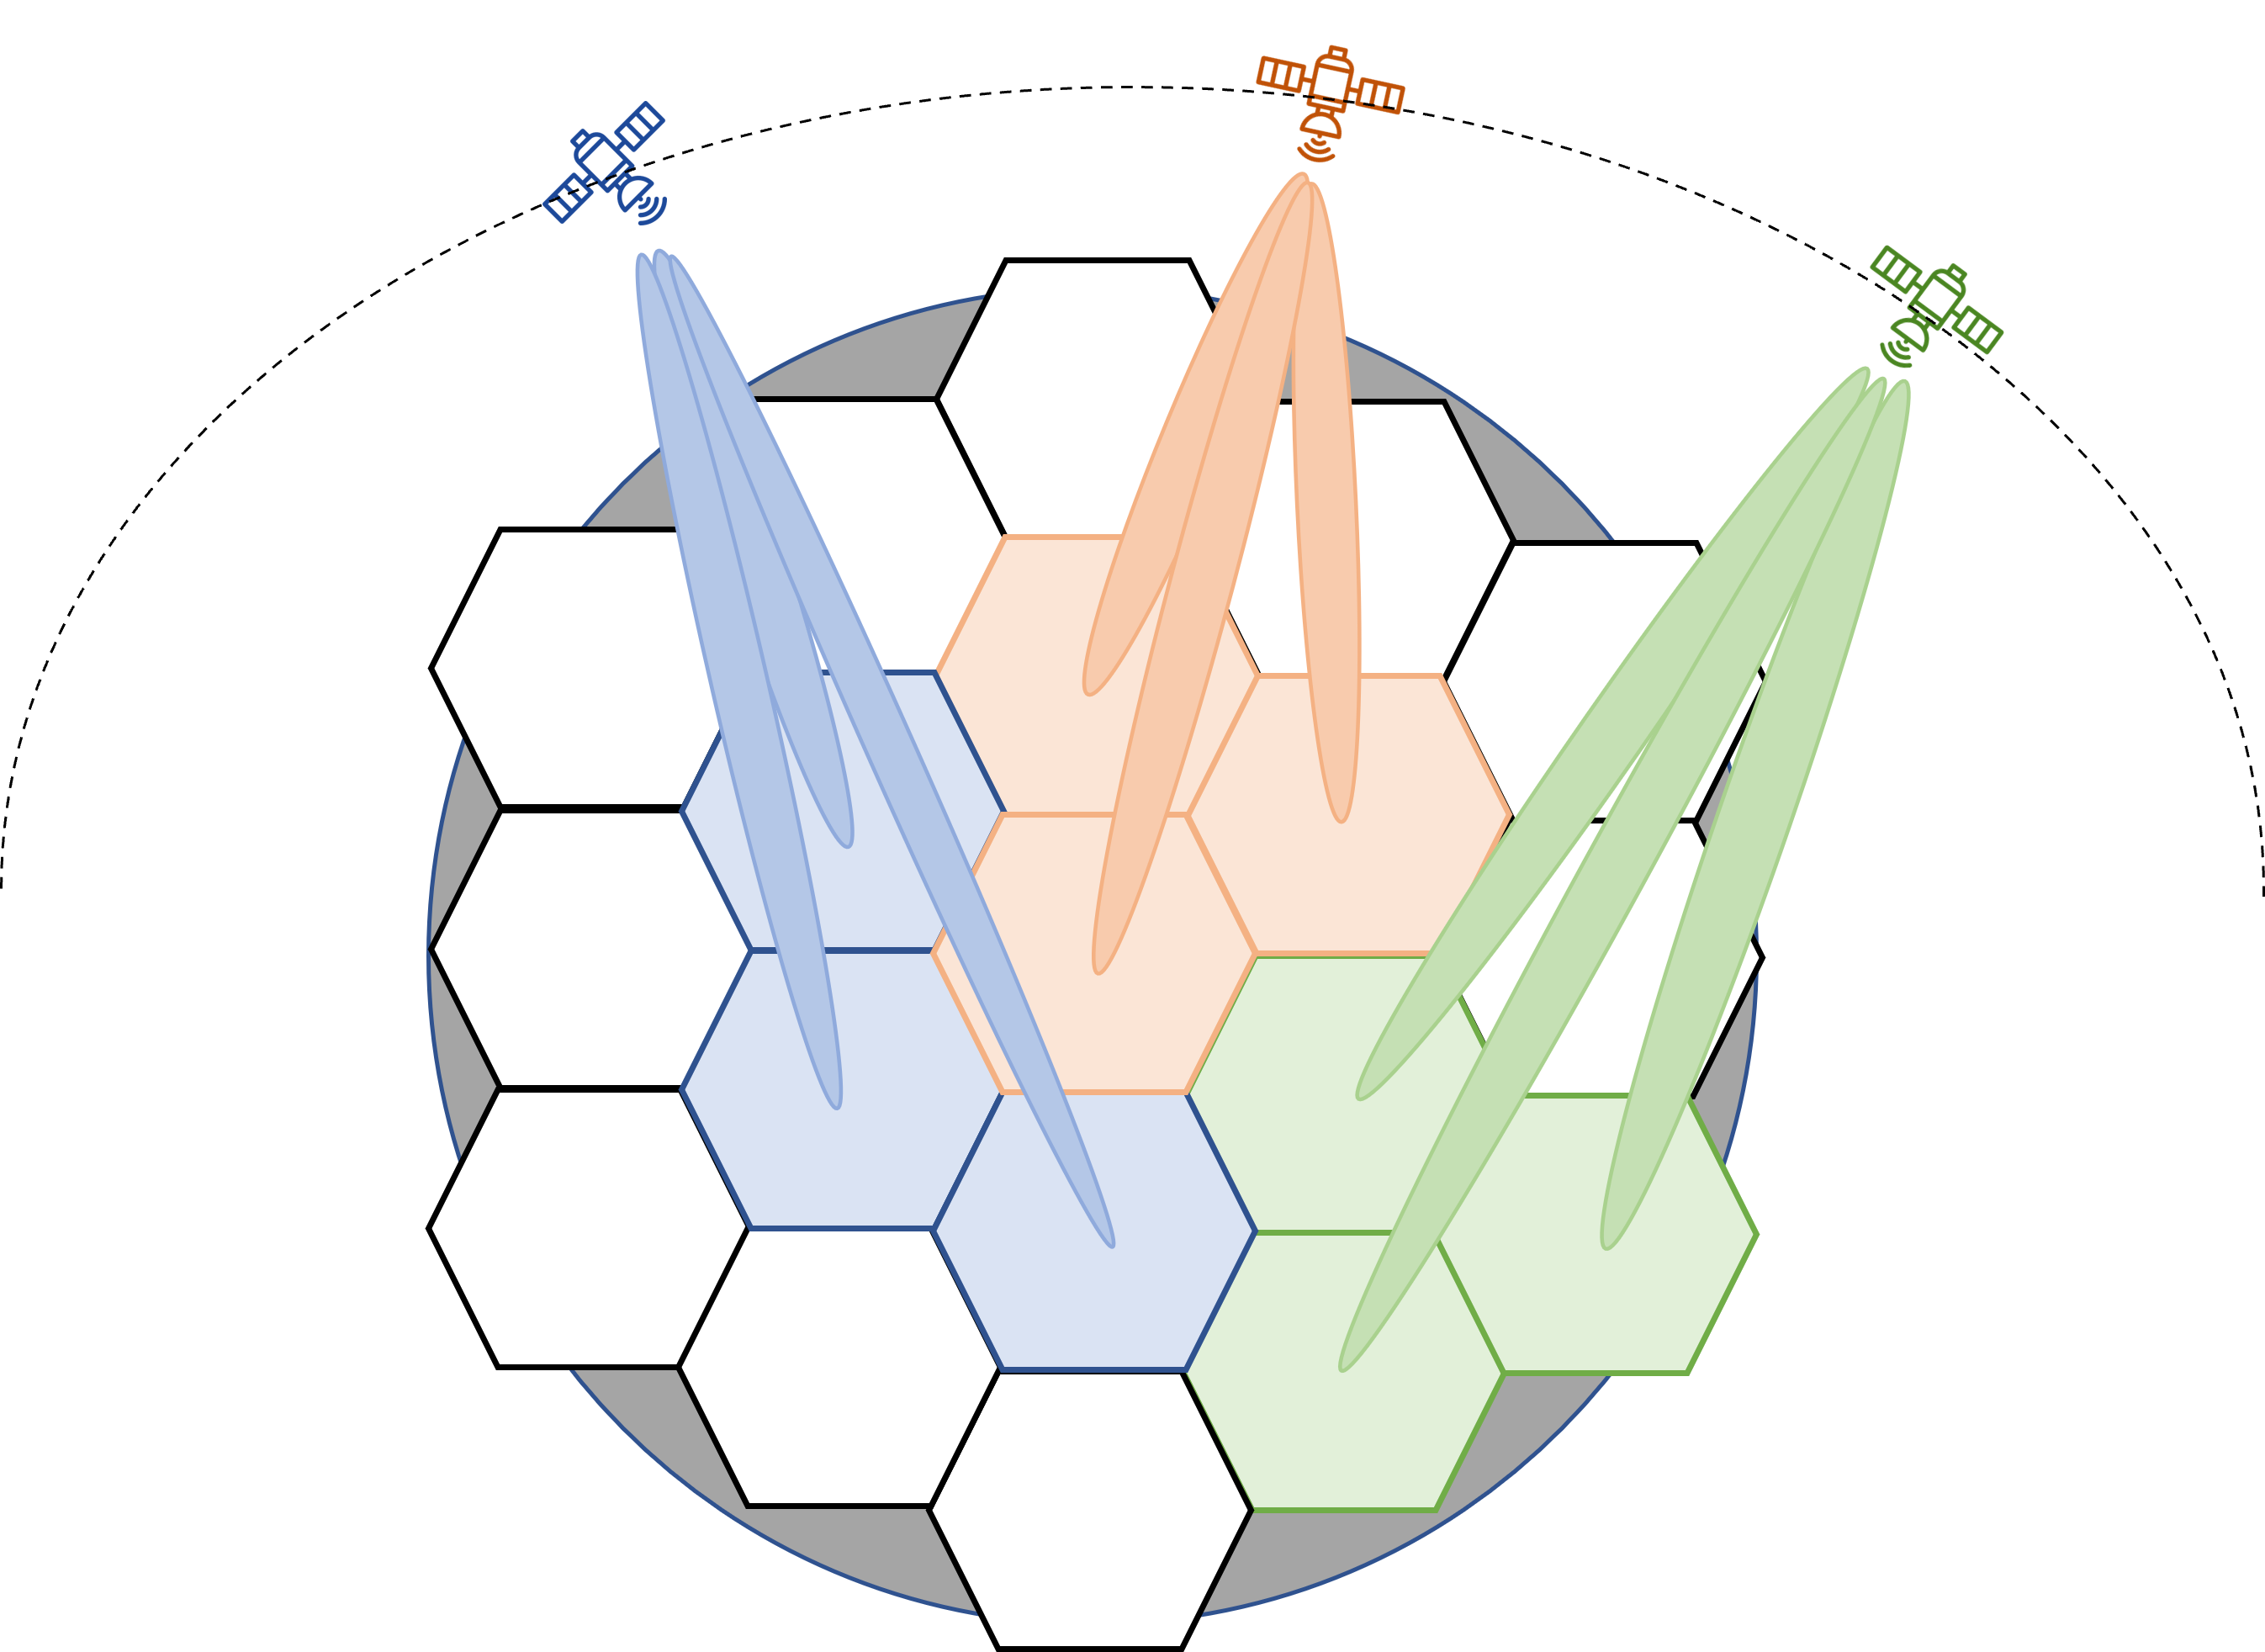
\includegraphics[width=0.8\textwidth]{satellites_cells.png}
    \caption{Illustration of satellite beams and cells}
    \label{fig_sat}
\end{figure}

\subsection{Channel Model}

In the LEO satellite system, the free space path loss model can be express as follows~\cite{Satellite-Multi-Beam}:
\begin{equation}
    L_{n,u} = \left(\frac{\lambda}{4\pi d_{n,u}}\right)^2
\end{equation}
where $\lambda$ is the wavelength,and d is the distance between the satellite n and the user u.
% In the LEO satellite system, the free space path loss defined by 3GPP protocol is as follows~\cite{38811}:
% \begin{equation}
% PL = 32.45 + 20\log_{10}(f_c) + 20\log_{10}(d),
% \end{equation}
% where $f_c$ is the carrier frequency and $d$ is the distance between the satellite and its serving cell position.
Also, we introduce the antenna radiation pattern in~\cite{Energy-Efficient}:
\begin{equation}
G(\theta) = G_{max} \left[ \frac{J_1\left(\mu(\theta)\right)}{2\mu(\theta)} 
+ 36 \frac{J_3\left(\mu(\theta)\right)}{\mu(\theta)^3} \right]^2,
\end{equation}
where $\theta$ represents the angle between the user and the beam center with respect to the satellite, $G_{max}$ is the maximum antenna gain, $\mu(\theta) = 2.07123\cdot \sin(\theta)/\sin(\theta_{3dB})$, 
where $\theta_{3dB}$ is the 3 dB half-power beamwidth angle of the antenna, and $J_1(\cdot)$ and $J_3(\cdot)$ represent the Bessel functions of the first kind of orders 1 and 3.

And considering the rain fading effect, we introduce a raining fading factor follows the Gaussian distribution $r~\sim \mathcal{N}(\mu, \sigma)$, where $\mu$ and $\sigma$
depends on the location, polarization, and elevation angle between UE and satellite~\cite{User-Scheduling}. 
Also, considering the payload (PL) oscillator phase noise $n_{theta}$ at the n-th satellite that follows a Gaussian distribution with zero mean and standard deviation 0.24:
\begin{equation}
    \hat\theta_{n,u} = \theta_{n,u} + n_{theta}
\end{equation}
Thus, The received power from the beam m of satellite n to the user u is:
\begin{equation}
    \hat{P}_{n,m,u} = P_{n,m} \cdot L_{n,u} \cdot G(\hat\theta_{n,u}) \cdot r_{n,u}
\end{equation}

\section{Problem Formulation}

Followed by 3GPP protocol~\cite{38331}, the supported SSB periodicity values are 
\{20, 40, 80, 160\} miliseconds. Here we define the SSB periodicity of each cell:
\begin{equation}
    T^{SSB}_{k}\in\{20, 40, 80, 160\}, \forall k
\end{equation}
We define the time duration of each slot as 160ms. 


    

